\section{Comparison between Octave and Ngspice results}
\label{sec:comparison}
\par Table \ref{tab:results_compar} shows, on the left, the values for the gain, and its deviation,
low and high cut-off frequency, central frequency, and its deviation, and input and output impedances,
found with Octave, and, on the right, using the Ngspice simulation tool.

\begin{table}[H]
  \centering
  \begin{tabular}{|l|r|}
      \hline    
      {\bf Name} & {\bf Value} \\ \hline
      \input{../mat/gain}
      $f_L$ & $723.431560$ \\ \hline 
$f_H$ & $1446.863119$ \\ \hline 
$f_0$ & $1023.086723$ \\ \hline 

      \input{../mat/freq_dev}
      $Z_I$ & $1707.106781$ \\ \hline 
$Z_O$ & $585.786438$ \\ \hline 

  \end{tabular}
\quad
  \begin{tabular}{|l|r|}
    \hline    
    {\bf Name} & {\bf Value} \\ \hline
    Output Voltage Gain dB & 266.369\\ \hline
Central Freq & 949.276\\ \hline
Low CO Freq & 453.95\\ \hline
Up CO Freq & 1985.08\\ \hline
Gain Deviation & 166.369\\ \hline
Gain Deviation dB & 8.50966\\ \hline
Central Freq Deviation &50.724\\ \hline
Bandwidth & 1531.13\\ \hline

    \input{../sim/freq_tab}
    \input{../sim/freq_dev_tab}
    zi & 5.638527e-01,-8.44302e-02\\ \hline

    zo & -1.00554e+01,1.184265e+00\\ \hline

  \end{tabular}
  \caption{Results for the gain, frequencies, input and output impedances.}
  \label{tab:results_compar}
\end{table}

\par All values presented, on both sides, were already annalised individually in both theoretical and
simulation contexts, Sections \ref{sec:analysis} and \ref{sec:simulation}. In this Section, our goal
is to determine the simmilarity between both.

\begin{figure}[H] \centering
  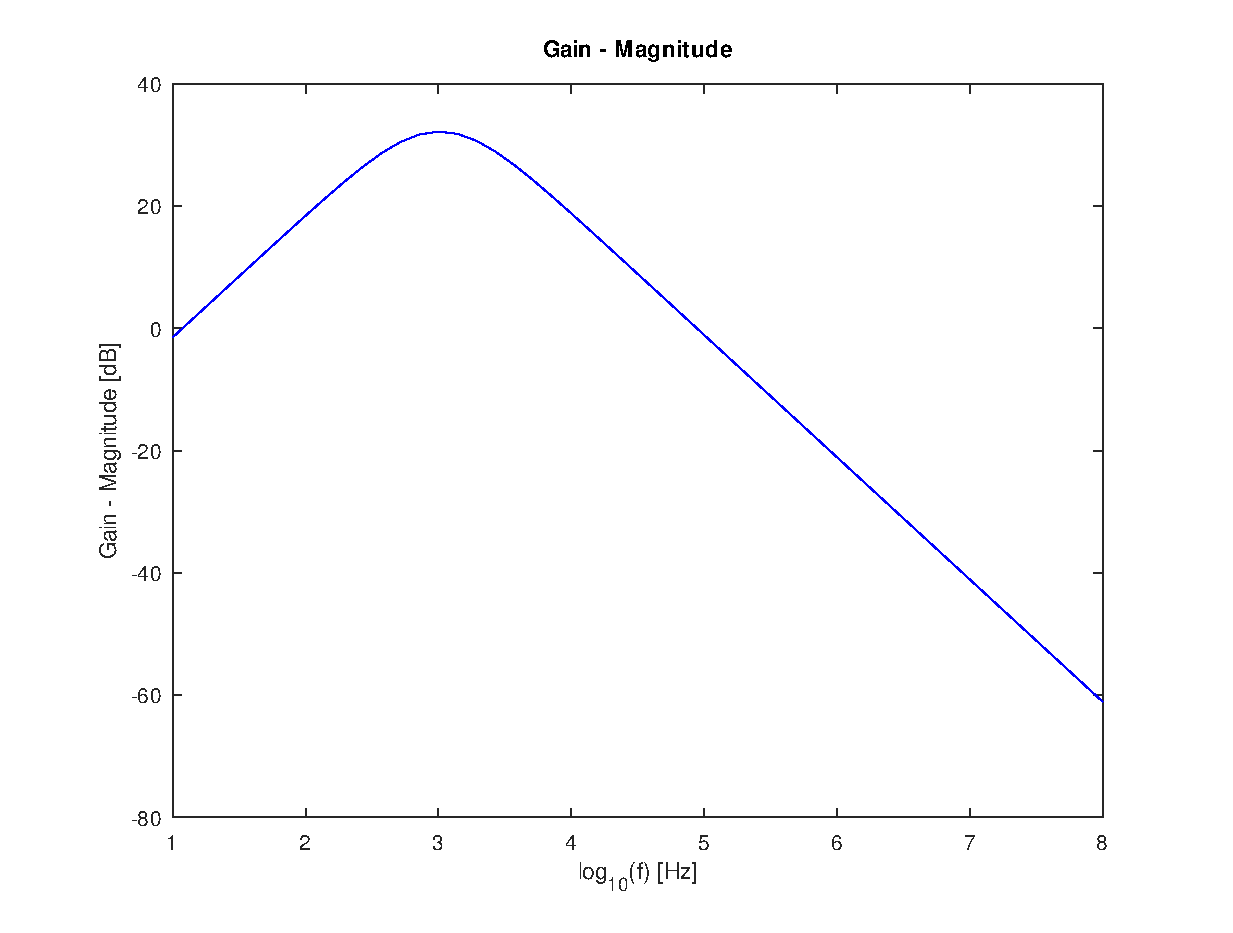
\includegraphics[width=0.8 \linewidth]{freq_db.eps}
  \caption{Gain Magnitude [dB] - Octave.}
  \label{fig:gain_compar}
\end{figure}

\begin{figure}[H] \centering
  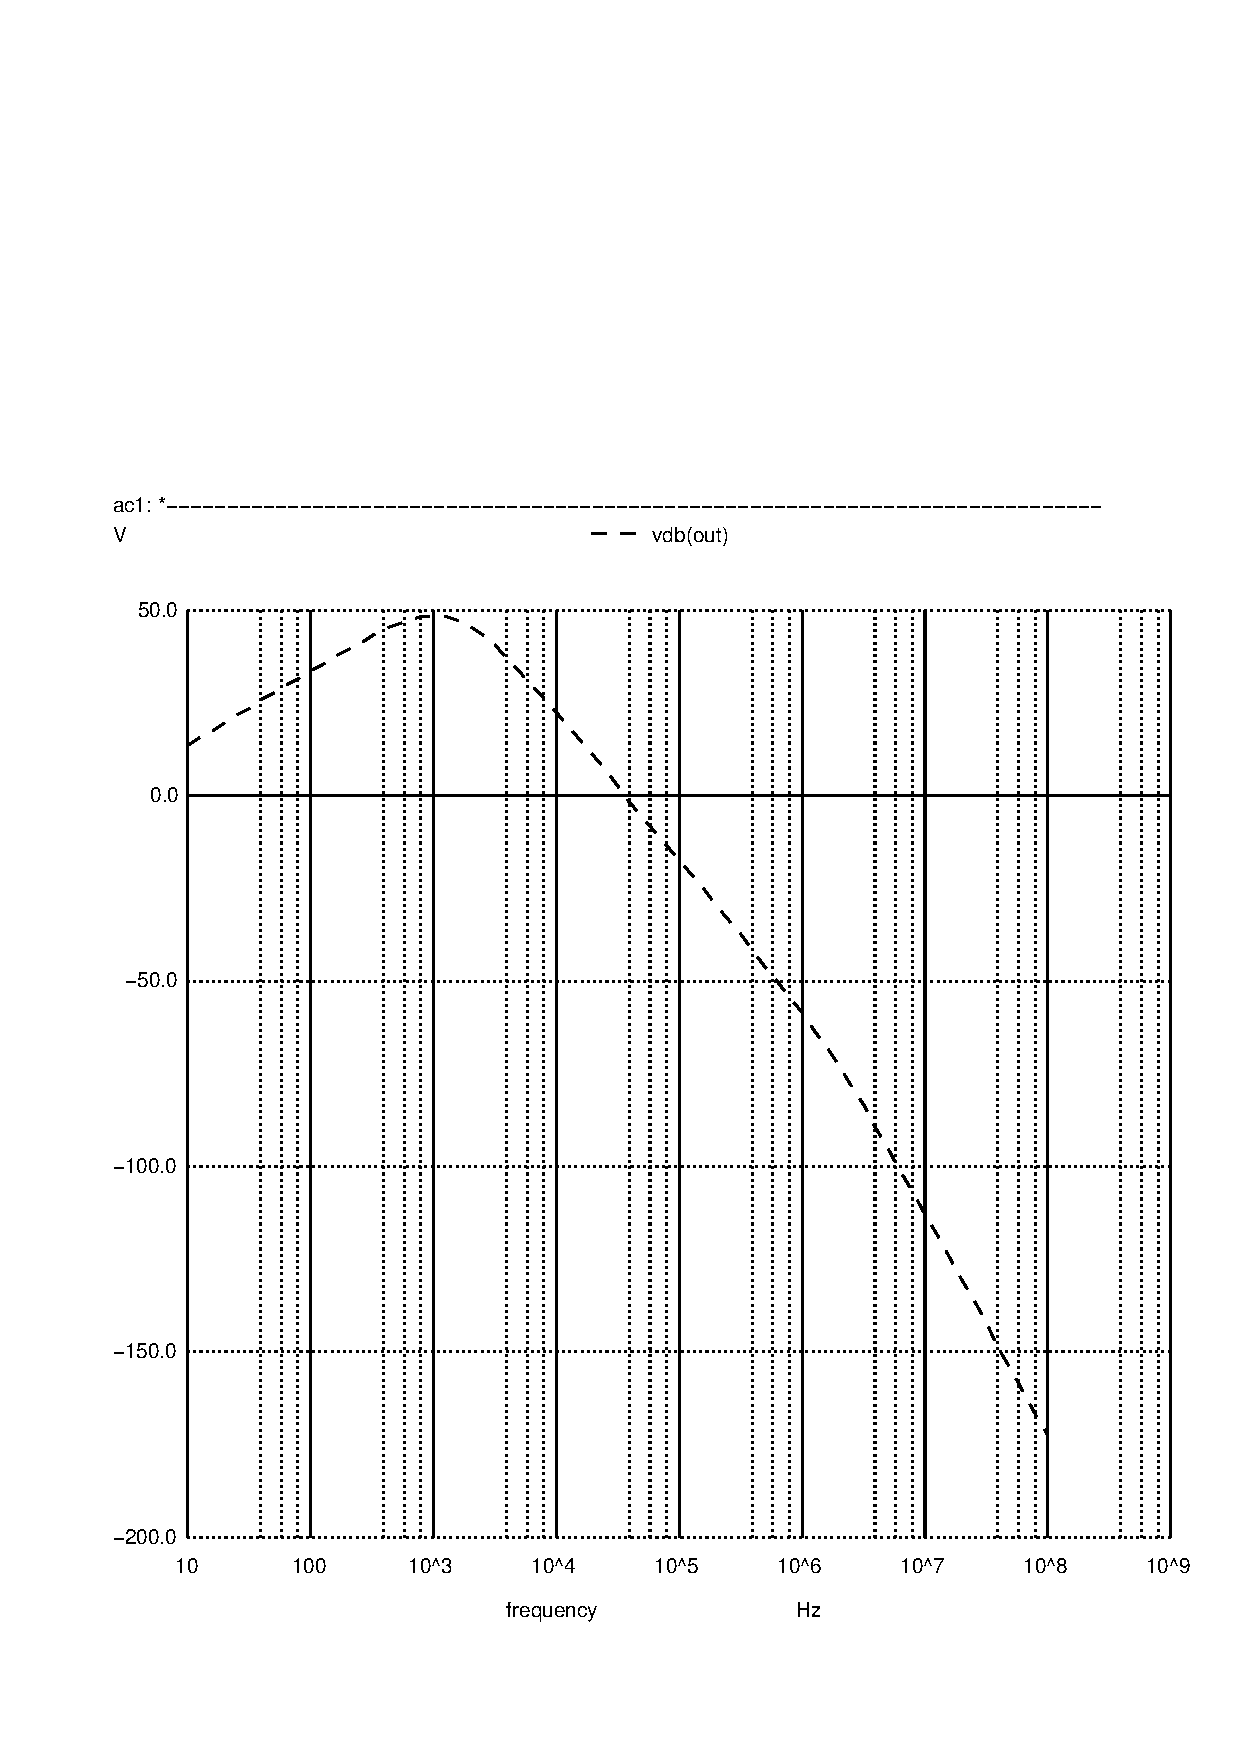
\includegraphics[clip, trim=1.3cm 1.3cm 0cm 7cm, width=0.6\linewidth]{vdb.pdf}
  \caption{Gain Magnitude [dB] - Ngspice.}
  \label{fig:vdb_compar}
\end{figure}


\begin{figure}[H] \centering
  \includegraphics[width=0.8 \linewidth]{freq_p_deg.eps}
  \caption{Gain Phase [deg] - Octave.}
  \label{fig:phase_compar}
\end{figure}

\begin{figure}[H] \centering
  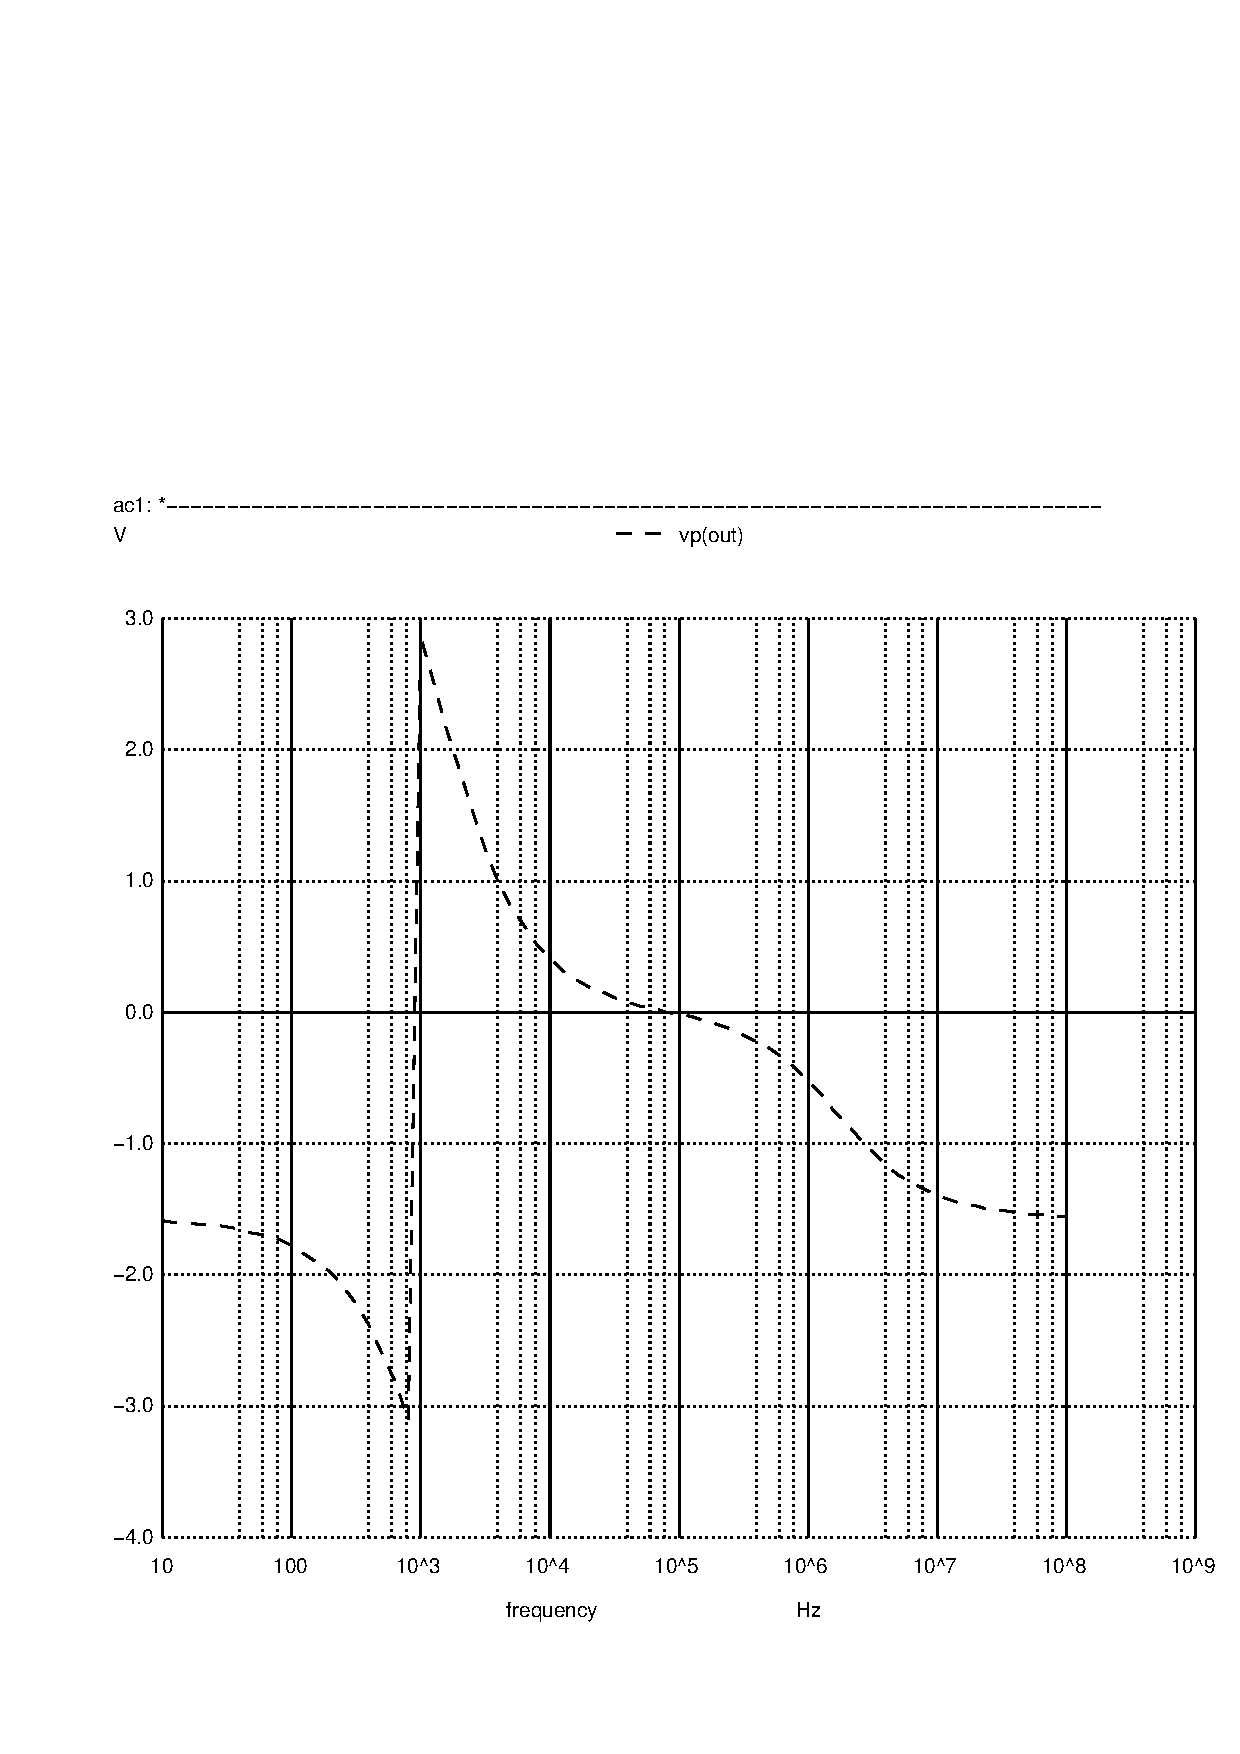
\includegraphics[clip, trim=1.3cm 1.3cm 0cm 7cm, width=0.6\linewidth]{vp.pdf}
  \caption{Gain Phase [deg] - Ngspice.}
  \label{fig:vp_compar}
\end{figure}

\par From the start, it is noticeable some discrepancies between the values, being the most obvious explanation
related to the fact that the Ngspice tool doesn't assume an ideal OP-AMP, using an approximated model, while
in the theoretical analysis provided by the Octave math tool it was assumed the ideal model. This affects
significantly both gain and central frequency, and its dependent values, such as their deviations, as one can
observe on Table \ref{tab:results_compar}.
\par Regarding the gain phase, one possible explanation is founded by the addition of two more poles by the
OPAMP model within the Ngspice simulation, which doesn't happen in the theoretical analysis, once it is used
an ideal OPAMP model. One more reason for this diference is due to Ngspice's graphical representation, which
frames the phase values between -90 and 90 degrees.
